\documentclass[10pt,a4paper]{article}
\usepackage{fontspec,polyglossia}
\setmainlanguage{russian}
\setmainfont{Times New Roman}
\usepackage{amsmath,amssymb,booktabs,tabularx,graphicx}
\usepackage[margin=17mm]{geometry}
\usepackage[hidelinks]{hyperref}
\usepackage{titlesec}
\titleformat{\section}{\large\bfseries}{}{0pt}{}
\titlespacing*{\section}{0pt}{8pt}{4pt}
\setlength{\parindent}{0pt}
\setlength{\parskip}{4pt}
\setlength{\emergencystretch}{3em}
\begin{document}
{\Large\bfseries MG при обучении классификатора MNIST}\par\medskip

29 сентября 2026. Проверка новой постановки после неудачного GAN-пилота.

\textbf{Итог.} Переход к фиксированной выборке для измерения loss частично помог. После снижения learning rate ковариационный effective rank колебаний весов снизился сильнее контроля во всех пяти новых запусках. MG обнаружил дополнительное снижение в четырёх из пяти, но медианный эффект относительно контроля всего 4,8\%. На окне 1024 шага результат лучше, однако это дополнительная проверка. \textbf{Устойчивое преимущество MG перед дешёвыми альтернативами пока не установлено.}

\section*{1. Кто учится, чему и зачем}

Обучается обычный классификатор рукописных цифр: на входе изображение, на выходе вероятности десяти классов. Практический мотив --- наблюдать, как меняются колебания параметров после уменьшения шага обучения. Хранить скалярный loss проще, чем всю историю весов. Проверяем, позволяет ли MG заметить изменение динамики по такому скаляру. Это диагностика заранее заданного изменения learning rate, не алгоритм его автоматического выбора.

\textbf{Данные.} MNIST, 2040 обучающих изображений: по 204 на класс, выбор без возвращения с seed 260929. Пиксели делятся на 255; усреднение непересекающихся блоков 2 на 2 уменьшает размер с 28 на 28 до 14 на 14. Аугментаций нет. Для мониторинга loss взяты фиксированные 100 изображений из официальной тестовой части, по 10 на класс. Они не участвуют в градиентных обновлениях. Оставшиеся 9900 служат для отдельной оценки accuracy. Полная тестовая accuracy уже записывалась при обучении, поэтому это не слепой финальный тест качества.

\textbf{Модель и обучение.} MLP: 196 входов, скрытые слои 64 и 32 с tanh, 10 выходов; всего 15 018 обучаемых весов и смещений. Loss --- средняя cross-entropy. SGD с momentum 0,9, batch size 64, выборка батча с возвращением, без weight decay. 4096 обновлений, начальный learning rate 0,1. Пять новых инициализаций: seeds 1--5; данные и наблюдатель одинаковы для всех.

\textbf{Парный контроль.} После 2048 обновлений создаются две ветви из одинаковых весов, momentum и состояния генератора батчей. В base шаг остаётся 0,1, в drop становится 0,01. Дальнейшие батчи совпадают. До развилки траектории побитово одинаковы. Таким образом, сравнивается эффект расписания шага, а не различие случайных обучений.

\section*{2. Что изменили относительно исходной попытки}

В пилоте на seed 0 проверены full-batch GD с шагами 1 и 3, а также SGD с momentum. Первый режим уже давал почти одномерную ковариационную траекторию; второй не обучил классификатор. В SGD независимый показатель снизился, но MG обычного minibatch loss вырос: отношение «после/до» 1,034 против 1,029 у контроля.

Причина для изменения измерения: при каждом новом батче меняются и веса, и сами изображения, на которых считается loss. Поэтому по сохранённым весам повторно рассчитали loss на фиксированных 100 изображениях. Это не меняло обучение. Выбор наблюдателя сделан по пилоту; затем зафиксирован перед seeds 1--5. Основной результат ниже --- исходный loss на фиксированной контрольной выборке, без удаления его тренда. Варианты с обучающей выборкой, проекцией весов и удалением тренда сохранены как дополнительные.

\newpage

\section*{3. Как независимо измеряли изменение динамики}

Каждый шаг сохраняет вектор весов до обновления; ему соответствует измеряемый loss. Окно содержит $W=512$ последовательных векторов; новое окно каждые 256 шагов. Из каждой координаты весов вычитаются среднее и линейный тренд по времени. Получается матрица остатков $X$ размера $512\times15018$. Основной независимый показатель:

\[
G=XX^\top,\qquad \mathrm{PR}=\frac{(\operatorname{tr}G)^2}{\sum_{i,j}G_{ij}^2}
=\frac{(\sum_i\lambda_i)^2}{\sum_i\lambda_i^2}.
\]

Здесь $\lambda_i$ --- собственные значения $G$. Падение PR означает более сильную концентрацию вариации в нескольких направлениях. Масштаб движения сам по себе PR не меняет; это проверено умножением на 10. Для расчёта PR не требуется разложение на собственные значения; спектры строятся отдельно для иллюстрации. Анализируется траектория весов, не полное состояние SGD с momentum. \textbf{PR не равен active dimension и не устанавливает истинное число компонент.}

\textbf{Что именно упрощается.} Основной результат относится к колебаниям после удаления локального линейного движения. Без удаления тренда PR не показывает более сильного снижения в drop ни в одной из пяти пар. Для PR обновлений согласование есть в трёх парах. Поэтому нельзя расширять вывод до уменьшения размерности всей траектории в любом смысле.

\textbf{MG.} В каждом окне loss стандартизуется; используется существующий код pooled nearest-neighbour estimator: embedding dimension $E=20$, delay $\tau=1$, 20 соседей, исключение временных соседей на расстоянии не более 39 шагов. Добавляется стандартный dither $10^{-9}$ с seed 123. Проверяется также $E=40$ при том же исключении. Ядро метода не изменялось. Ни одно основное окно не помечено как численно вырожденное, но отношение оценок при $E=40$ и $E=20$ достигает 2,08: устойчивость абсолютной размерности не подтверждена.

\textbf{Как сравниваем.} Для каждого показателя $m$ берём медиану пяти окон до изменения шага (концы 1024, 1280, 1536, 1792, 2048) и пяти поздних окон (3072, 3328, 3584, 3840, 4096). Определяем:

\[
r_m=\frac{\operatorname{median}(m_{\mathrm{late}})}{\operatorname{median}(m_{\mathrm{early}})},\qquad
q_m=\frac{r_m^{\mathrm{drop}}}{r_m^{\mathrm{base}}}.
\]

Значение $q_m<1$ означает более сильное снижение относительно контроля. Простого падения во времени недостаточно: оно встречается и без изменения шага. Окна перекрываются; это не независимые повторы. Единица сравнения --- пара ветвей одной инициализации.

\section*{4. Результаты всех пяти новых инициализаций}

\begin{center}\small
\begin{tabularx}{\linewidth}{l>{\raggedright\arraybackslash}X>{\raggedright\arraybackslash}X>{\raggedright\arraybackslash}X>{\raggedright\arraybackslash}X}
\toprule
Seed & PR: base / drop & MG: base / drop & $q_{\mathrm{PR}}$ & $q_{\mathrm{MG}}$ \\
\midrule
1 & 1,079 / 0,785 & 0,805 / 0,766 & 0,728 & 0,952 \\
2 & 0,876 / 0,666 & 0,805 / 0,809 & 0,761 & 1,005 \\
3 & 1,174 / 0,905 & 0,987 / 0,813 & 0,770 & 0,824 \\
4 & 0,814 / 0,635 & 0,848 / 0,766 & 0,780 & 0,903 \\
5 & 0,888 / 0,727 & 0,828 / 0,823 & 0,818 & 0,993 \\
\bottomrule\end{tabularx}\end{center}

В столбцах base / drop указаны $r_m$, не абсолютные значения. Медиана $q_{\mathrm{PR}}=0,770$, а $q_{\mathrm{MG}}=0,952$. У MG неверный знак в seed 2 и почти нулевой дополнительный эффект в seed 5. Accuracy на 9900 изображениях --- 91,5--92,4\%; снижение шага не улучшило итоговую accuracy в этих парах. Полученный сигнал касается динамики, а не доказанного улучшения обобщения.

\newpage

\section*{5. Траектории, спектр и устойчивость результата}

\begin{center}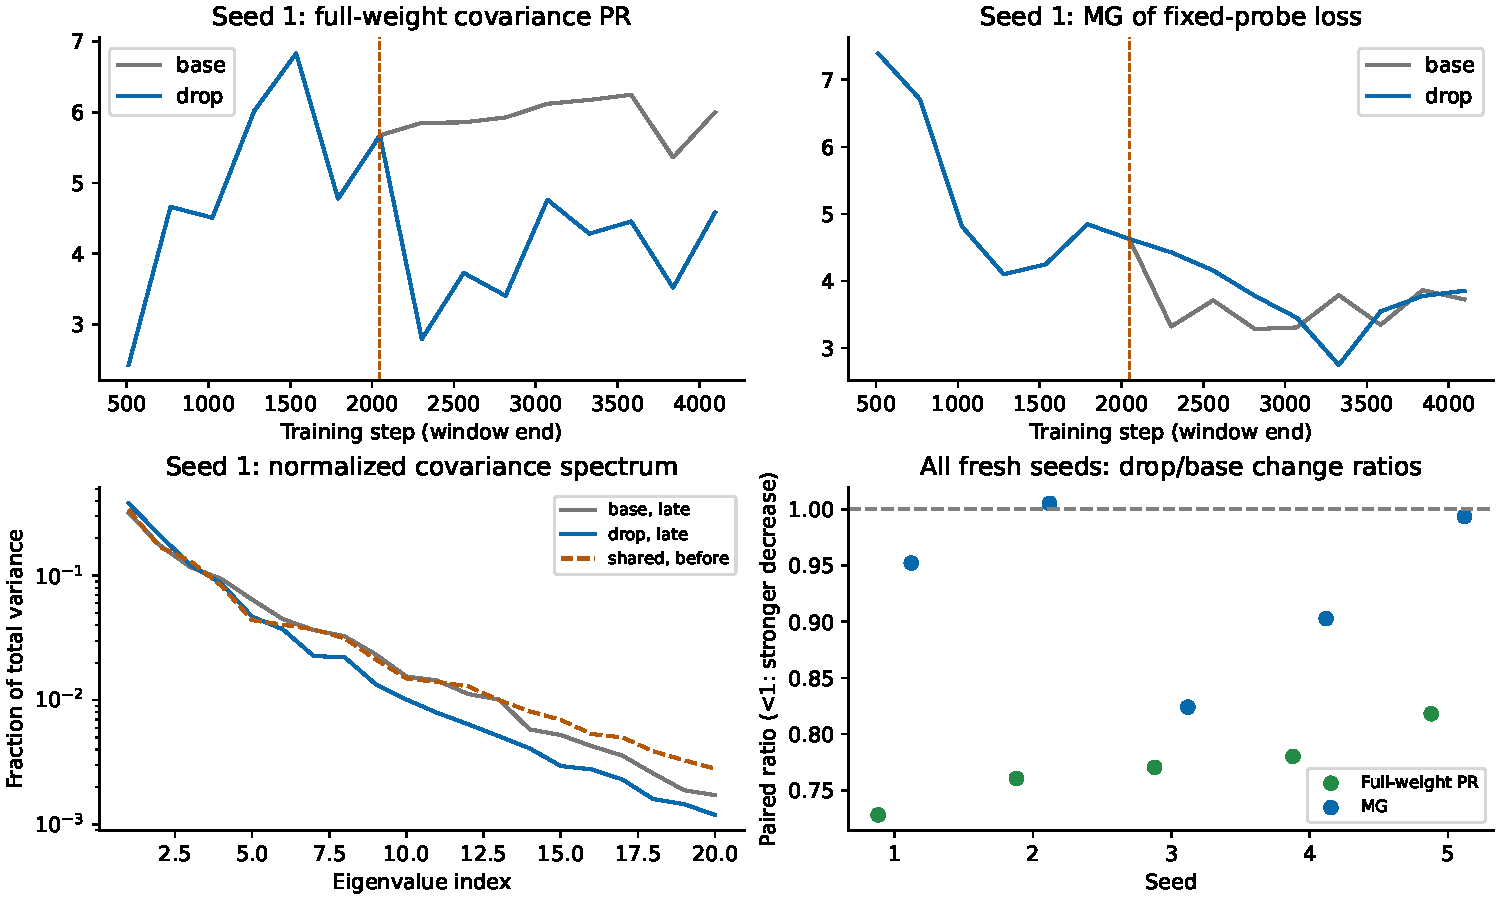
\includegraphics[width=\linewidth,height=.30\textheight,keepaspectratio]{results.pdf}\end{center}

Сверху: один и тот же seed 1, PR колебаний всех весов и MG фиксированного loss. Вертикаль --- изменение шага; точка показывает конец окна. Снизу слева: первые 20 собственных значений, делённые на сумму всех 512; сравниваются окна, заканчивающиеся на шагах 2048 и 4096. Справа --- все пять пар. Seed 1 показан как первая инициализация подтверждающей серии, без выбора наиболее удачного графика. У MG видимого устойчивого разрыва между ветвями на этом примере нет.

\textbf{Зависимость от настроек.} Таблица ниже меняет только параметры MG на уже полученных запусках; основной независимый критерий остаётся PR с окном 512. Эти проверки не являются новой подтверждающей серией и не устанавливают оптимальное окно.

\begin{center}\small
\begin{tabularx}{\linewidth}{>{\raggedright\arraybackslash}Xrr}
\toprule
Окно и delay MG & Пар с $q_{\mathrm{MG}}<1$ & Медиана $q_{\mathrm{MG}}$ \\
\midrule
256, $\tau=1$ & 2 из 5 & 1,024 \\
512, $\tau=1$ --- основной & 4 из 5 & 0,952 \\
1024, $\tau=1$ & 5 из 5 & 0,880 \\
512, $\tau=4$ & 2 из 5 & 1,035 \\
\bottomrule\end{tabularx}\end{center}

Длинное окно даёт перспективный сигнал: около 12\% дополнительного снижения по отношению к контролю. Но оно сильнее усредняет время. Это результат проверки чувствительности после основной серии, поэтому представлять его как заранее выбранный успешный протокол нельзя.

\textbf{Другие проверки.} Умножение скаляра на 10 не меняет MG в пределах численной точности. Проверены также сглаживание по 8 точкам и три IAAFT-суррогата на раннем и позднем окнах каждой ветви. Последние сохраняют распределение значений и приближённо спектр. Отношения MG исходного ряда к медиане суррогатов имеют обе стороны от единицы; устойчивого разделения нет. Это не подтверждает восстановление особой нелинейной геометрии.

\textbf{Дешёвые конкуренты.} PR по 128 фиксированным случайным координатам весов обнаружил более сильное снижение во всех пяти парах: медиана $q=0,755$. Нормированная спектральная энтропия loss --- также в пяти парах, медиана $q=0,718$. Стандартное отклонение и частота пересечений удалённого линейного тренда тоже меняются во всех пяти парах. Это другие характеристики, не заменители intrinsic dimension, но в данной задаче наличие изменения можно установить без MG. Превосходство MG по диагностической полезности здесь не показано.

\newpage

\section*{6. Сколько стоит наблюдение}

CPU Intel Core i5-12500H; один вычислительный поток для сравнения, семь повторов после прогрева, ниже медианы. Для одного окна 512 шагов: полный PR --- 225,1 мс; PR по 128 весам --- 6,2 мс; MG --- 11,5 мс; MG вместе с повтором при $E=40$ --- 29,3 мс. Простой набор скалярных статистик --- 0,45 мс. Передача данных на GPU не измерялась.

Однако фиксированный loss ещё нужно получить: forward на 100 изображениях стоит около 0,150 мс на каждый шаг. Поэтому сравнение только 11,5 против 225,1 мс завышает практический выигрыш. Для всей траектории 4096 шагов с 15 перекрывающимися окнами складываем стоимость наблюдений, получаемых один раз на шаг, и анализа всех окон:

\begin{center}\small
\begin{tabularx}{\linewidth}{>{\raggedright\arraybackslash}Xrr}
\toprule
Вариант мониторинга & Анализ 15 окон, с & С наблюдениями, с \\
\midrule
PR по всем 15 018 весам & 3,377 & 3,582 \\
PR по 128 весам & 0,093 & 0,205 \\
MG & 0,173 & 0,787 \\
MG и проверка $E=40$ & 0,439 & 1,053 \\
Простые статистики того же loss & 0,007 & 0,621 \\
\bottomrule\end{tabularx}\end{center}

Это \textbf{оценка накладных расходов из измеренных компонентов}, не время отдельного онлайн-запуска от начала до конца. Для весов учтено копирование в массивы RAM; для loss --- дополнительный forward. Запись на диск, отдельное построение спектров, загрузка данных и само обучение не включены. Замеры относятся к одному CPU и данной небольшой модели. Обучение и повторное вычисление наблюдателей выполнялись отдельно; офлайн-перенос сохранённых весов в модель не является необходимой стоимостью онлайн-мониторинга.

При таких условиях MG с проверкой быстрее полного PR примерно в 3,4 раза, \textbf{но медленнее PR по 128 весам примерно в 5,1 раза}. Сам MG без проверки быстрее полного PR примерно в 4,5 раза. Это не демонстрация превосходства над всеми практически применимыми методами.

Для хранения всей траектории нужно около 235 MiB в float32. Один скаляр float64 на шаг --- 32 KiB; 128 координат float32 --- 2 MiB. Здесь преимущество скалярного лога по объёму данных очевидно, но цена его получения и чувствительность к выбору наблюдателя остаются существенными.

\section*{7. Что можно утверждать и что делать с результатом}

\textbf{Подтверждено:} при реальном обучении распознаванию цифр после снижения learning rate вариация весов вокруг локального линейного тренда концентрируется в меньшем числе направлений. Фиксированный loss позволяет MG частично обнаруживать сопутствующее изменение; исходный minibatch loss был менее надёжен. Все пять новых инициализаций сохранены, неудачные случаи не исключены.

\textbf{Не подтверждено:} универсальное упрощение всей системы, точное число active components, преимущество MG перед простыми метриками, перенос на большие CV/NLP-модели, автоматическое управление обучением. Рекуррентность и условия теоретической интерпретации здесь не установлены.

\textbf{Рекомендация для статьи:} пока использовать как дополнительный эксперимент о выборе наблюдателя, устойчивости и стоимости. Не делать его главным доказательством практического превосходства. Вариант с окном 1024 заслуживает отдельной заранее зафиксированной проверки на новых запусках и более содержательной задаче, с сохранением дешёвых конкурентов.

Код, исходные скалярные логи, итоговые веса, спектры, все таблицы, протокол выбора и инструкции воспроизведения приложены. Большие полные траектории сохранены локально; в компактный архив не входят и воспроизводятся скриптами.
\end{document}